\documentclass[11pt,letterpaper]{article}

\usepackage[utf8]{inputenc}
\usepackage[T1]{fontenc}
\usepackage{lmodern}
\usepackage[letterpaper,margin=2.15cm]{geometry}
\usepackage{amsmath}
\usepackage{booktabs}
\usepackage{tabularx}
\usepackage{longtable}
\usepackage{xcolor}
\usepackage{graphicx}
\usepackage{float}
\usepackage{hyperref}

\definecolor{azulprofundo}{HTML}{123047}
\definecolor{azullago}{HTML}{167D9A}
\definecolor{aguamarina}{HTML}{47B8A6}
\definecolor{naranja}{HTML}{D5793D}
\definecolor{gristexto}{HTML}{405963}
\hypersetup{colorlinks=true,linkcolor=azullago,urlcolor=azullago,citecolor=azullago}
\graphicspath{{../outputs/figures/}{outputs/figures/}}
\setlength{\parindent}{0pt}
\setlength{\parskip}{0.58em}
\setlength{\emergencystretch}{2em}
\pagestyle{plain}
\renewcommand{\abstractname}{Resumen ejecutivo}
\renewcommand{\tablename}{Tabla}
\renewcommand{\figurename}{Figura}
\renewcommand{\refname}{Referencias}

\newcommand{\CYA}{\textsc{cya}}
\newcommand{\alerta}[1]{%
  \begin{center}\fcolorbox{naranja}{white}{\parbox{0.91\textwidth}{#1}}\end{center}}

\title{\vspace{-1.4cm}\color{azulprofundo}\textbf{Monitoreo satelital de señales asociadas con cianobacterias}\\[0.3em]
\Large Lagos Atitlán y Amatitlán, Guatemala\\[0.45em]
\large Laboratorio 4 --- Análisis geoespacial y sensores remotos}
\author{Grupo 1\\[0.35em]
Jorge Gabriel Palacios Sales --- 231385\\
Pablo Daniel Barillas Moreno --- 22193\\
Roberto Emiliano Otoniel --- 23968\\[0.35em]
CC3084 --- Data Science}
\date{Agosto de 2026}

\begin{document}
\maketitle

\begin{abstract}
Se analizaron 22 imágenes Sentinel--2 L2A, once por lago, adquiridas entre enero de 2025 y julio de 2026. Mediante Copernicus Data Space Ecosystem se calcularon NDVI, NDWI y el proxy de cianobacterias del modelo Se2WaQ, descargando únicamente las bandas necesarias. Amatitlán presentó una señal mucho más intensa, extensa y persistente: seis fechas cubrieron al menos 10\% del lago con \CYA{} mayor o igual que 40 y la extensión máxima llegó a 97.50\%. Atitlán no registró fechas bajo ese criterio; su máximo calculado fue 3.14\%, pero corresponde a una imagen con una discontinuidad de tesela y se interpreta con cautela. La máxima mediana robusta de ambos lagos ocurrió el 13 de abril de 2026: 262.24 en Amatitlán y 2.57 en Atitlán. Los resultados describen una respuesta espectral útil para priorizar vigilancia, no una confirmación de células, toxinas ni riesgo sanitario. Se requiere validación con mediciones de campo.
\end{abstract}

\alerta{\textbf{Mensaje para la gestión ambiental.} El producto \CYA{} es un modelo empírico satelital expresado en $10^3$ células/ml. No sustituye el conteo de laboratorio ni demuestra toxicidad. Su valor está en reconocer contrastes espaciales y temporales que orienten muestreos de campo.}

\section{Problema y objetivo}

Las floraciones de cianobacterias pueden reducir el oxígeno, alterar el ecosistema y afectar actividades recreativas, turísticas y de abastecimiento. La observación satelital permite revisar grandes superficies en fechas repetidas, pero responde a propiedades ópticas de la superficie y está condicionada por nubes, sombras y la calibración del modelo.

El objetivo fue describir la evolución temporal y espacial del proxy \CYA{} en Atitlán y Amatitlán, relacionarlo con NDVI y NDWI, comparar los dos lagos y explorar extensión, persistencia, distribución y posible estacionalidad. Las interpretaciones se sustentan en las estadísticas y mapas generados; las explicaciones ambientales se presentan como hipótesis compatibles con literatura, no como causalidad demostrada.

\section{Datos y delimitación espacial}

Se utilizó Sentinel--2 L2A mediante la API openEO de Copernicus. La guía estableció once fechas por lago y se conservaron exactamente. Los GeoJSON entregados por el curso reproducen las cajas rectangulares de las coordenadas publicadas: 121.7 km$^2$ para Amatitlán y 474.2 km$^2$ para Atitlán. Estas geometrías limitan la consulta, pero no siguen la orilla.

Para calcular porcentajes del lago se usaron contornos del espejo de agua obtenidos de OpenStreetMap, relaciones 11018382 y 5781818, con áreas proyectadas aproximadas de 15.02 km$^2$ y 124.70 km$^2$, respectivamente. Así se distingue la \emph{extensión oficial de búsqueda} del \emph{polígono usado como denominador ambiental}.

\begin{table}[H]
\centering
\caption{Diseño del conjunto de observaciones.}
\begin{tabularx}{\textwidth}{lccX}
\toprule
\textbf{Lago} & \textbf{Fechas} & \textbf{Área de recorte} & \textbf{Cobertura válida observada} \\
\midrule
Amatitlán & 11 & 15.02 km$^2$ & 77.68--97.53\% \\
Atitlán & 11 & 124.70 km$^2$ & 43.21--98.38\% \\
\bottomrule
\end{tabularx}
\end{table}

\section{Procesamiento e índices}

Se solicitaron únicamente B02 (azul), B03 (verde), B04 (rojo), B08 (infrarrojo cercano) y SCL (clasificación de escena). Los productos se generaron a 20 m en UTM zona 15N. Las reflectancias se obtuvieron multiplicando los enteros de Sentinel--2 por 0.0001.

\begin{align}
\mathrm{NDVI} &= \frac{B08-B04}{B08+B04}, \\
\mathrm{NDWI} &= \frac{B03-B08}{B03+B08}, \\
\mathrm{CYA} &= 115530.31\left(\frac{B03\,B04}{B02}\right)^{2.38}.
\end{align}

La fórmula \CYA{} coincide con Se2WaQ \cite{se2waq,potes2018}. El script define el fondo mediante NDWI y presenta \CYA{} cuando $\mathrm{NDWI}\geq0$; este criterio se reprodujo. Se excluyeron SCL 0, 1, 3, 8, 9, 10 y 11, además de reflectancias no positivas. Los píxeles excluidos permanecieron como datos faltantes y nunca se reemplazaron por cero.

La escala gráfica Se2WaQ termina en 100, pero la fórmula no. Para cumplir con el análisis temporal se calculó la media aritmética cruda de \CYA{} por lago y fecha. Como los valores extremos pueden elevarla, se presenta junto con la mediana y percentiles crudos. La media limitada a 0--100 se conserva solo como diagnóstico de saturación. Se definió \CYA{} $\geq40$ como señal alta porque 40 es un corte publicado en la rampa Se2WaQ; no es un límite sanitario. También se repitió el cálculo con 20 y 60.

\section{Control de calidad}

Las 22 observaciones contienen NDVI, NDWI y \CYA{} con rejillas compatibles. Tres fechas tuvieron menos de 80\% de cobertura válida: Amatitlán 28-04-2026 (77.68\%), Atitlán 18-01-2025 (43.21\%) y Atitlán 12-02-2026 (77.08\%). Además, Atitlán 17-07-2025 presenta una discontinuidad rectangular occidental compatible con un límite de tesela. La fecha se conserva para trazabilidad, pero ese parche no se interpreta como patrón natural ni se usa para seleccionar mapas representativos.

La guía anticipa aproximadamente 57.1\% de cobertura válida para Amatitlán el 07-02-2026. Nuestro producto openEO alcanza 89.08\% sobre el contorno fino del espejo de agua después de aplicar SCL y $\mathrm{NDWI}\geq0$. Las cifras no usan necesariamente el mismo denominador ni la misma composición de teselas: la guía describe la cobertura de la imagen de referencia, mientras este flujo mide los píxeles válidos del mosaico exportado dentro del polígono acuático. Por ello se reporta el 89.08\% observado en el producto analizado y se conserva explícitamente la cifra de la guía para trazabilidad.

\alerta{Las líneas temporales conectan fechas separadas e irregulares. No implican que el valor haya cambiado de manera lineal entre adquisiciones.}

\section{Análisis temporal}

\begin{figure}[H]
\centering
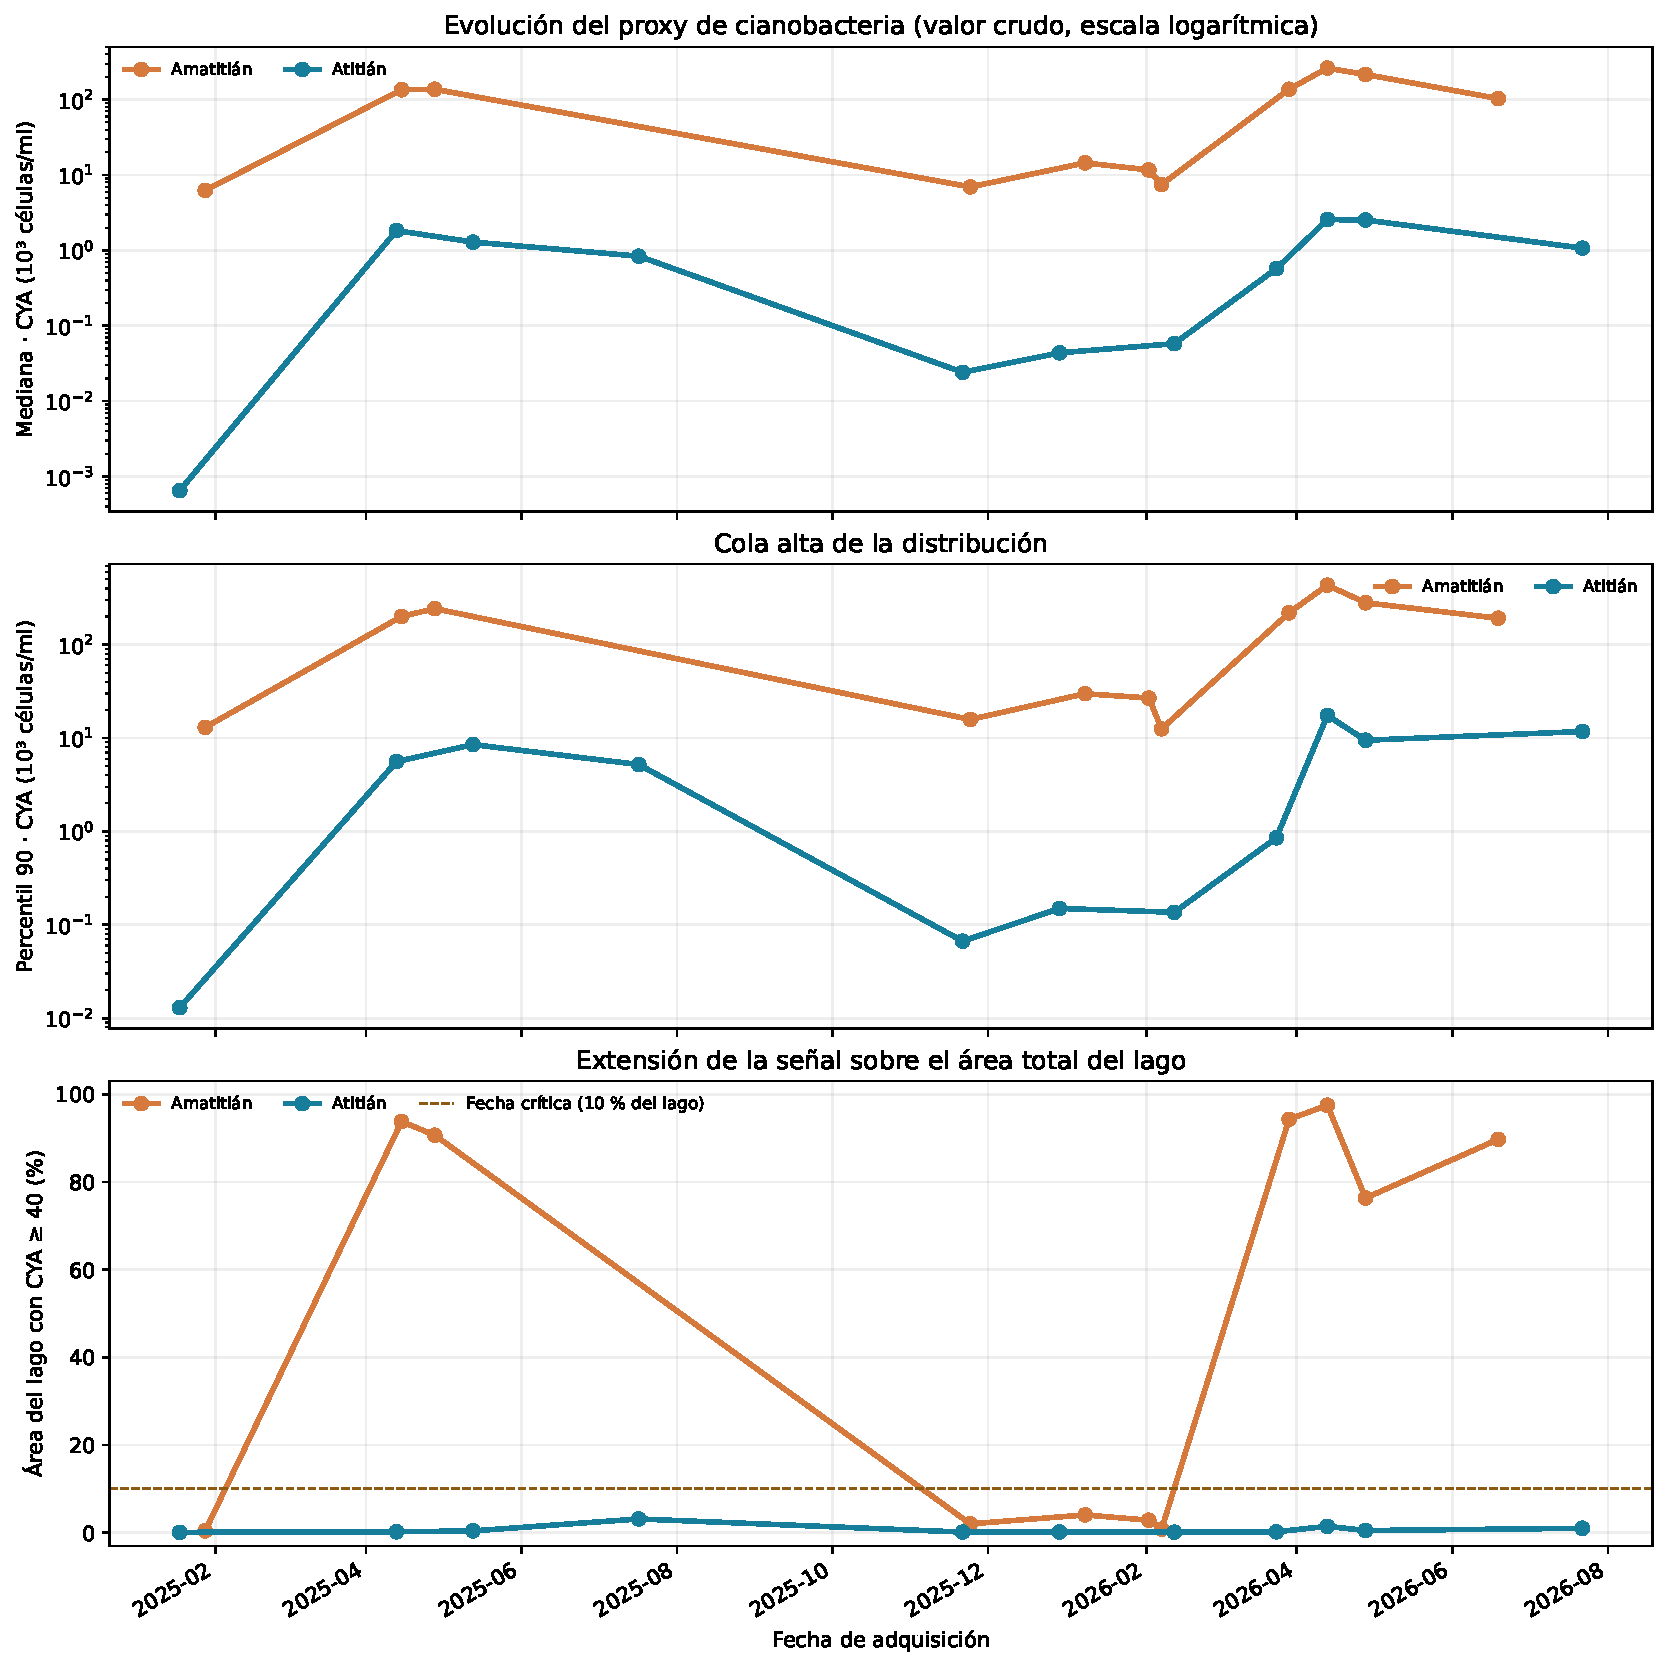
\includegraphics[width=\textwidth]{serie_temporal_cya.pdf}
\caption{Media aritmética y mediana por lago y fecha, percentil 90 y porcentaje del área total del lago con \CYA{} $\geq40$. La escala logarítmica permite comparar lagos con órdenes de magnitud distintos.}
\label{fig:temporal}
\end{figure}

Amatitlán alternó dos regímenes visibles (Figura~\ref{fig:temporal}). Enero de 2025, noviembre de 2025 y enero--febrero de 2026 mostraron extensiones bajas. En abril de 2025 y desde el 29 de marzo hasta el 19 de junio de 2026 la señal fue generalizada. La máxima media aritmética y la máxima mediana ocurrieron el 13-04-2026, con 275.03 y 262.24, respectivamente; el percentil 90 fue 433.04 y 97.50\% del lago superó 40.

Seis fechas se clasificaron como críticas por cubrir al menos 10\% del lago: 15-04-2025, 28-04-2025, 29-03-2026, 13-04-2026, 28-04-2026 y 19-06-2026. El criterio identifica extensión, no toxicidad.

Atitlán permaneció varios órdenes de magnitud por debajo. Su máxima media aritmética fue 15.32 el 17-07-2025, impulsada por valores extremos asociados con el artefacto de esa escena; la máxima mediana robusta fue 2.57 el 13-04-2026 y su percentil 90 llegó a 17.43. El mayor porcentaje calculado, 3.14\% el 17-07-2025, también está afectado por el artefacto mencionado. Ninguna fecha alcanzó el criterio crítico de 10\%.

\section{Análisis espacial}

\begin{figure}[H]
\centering
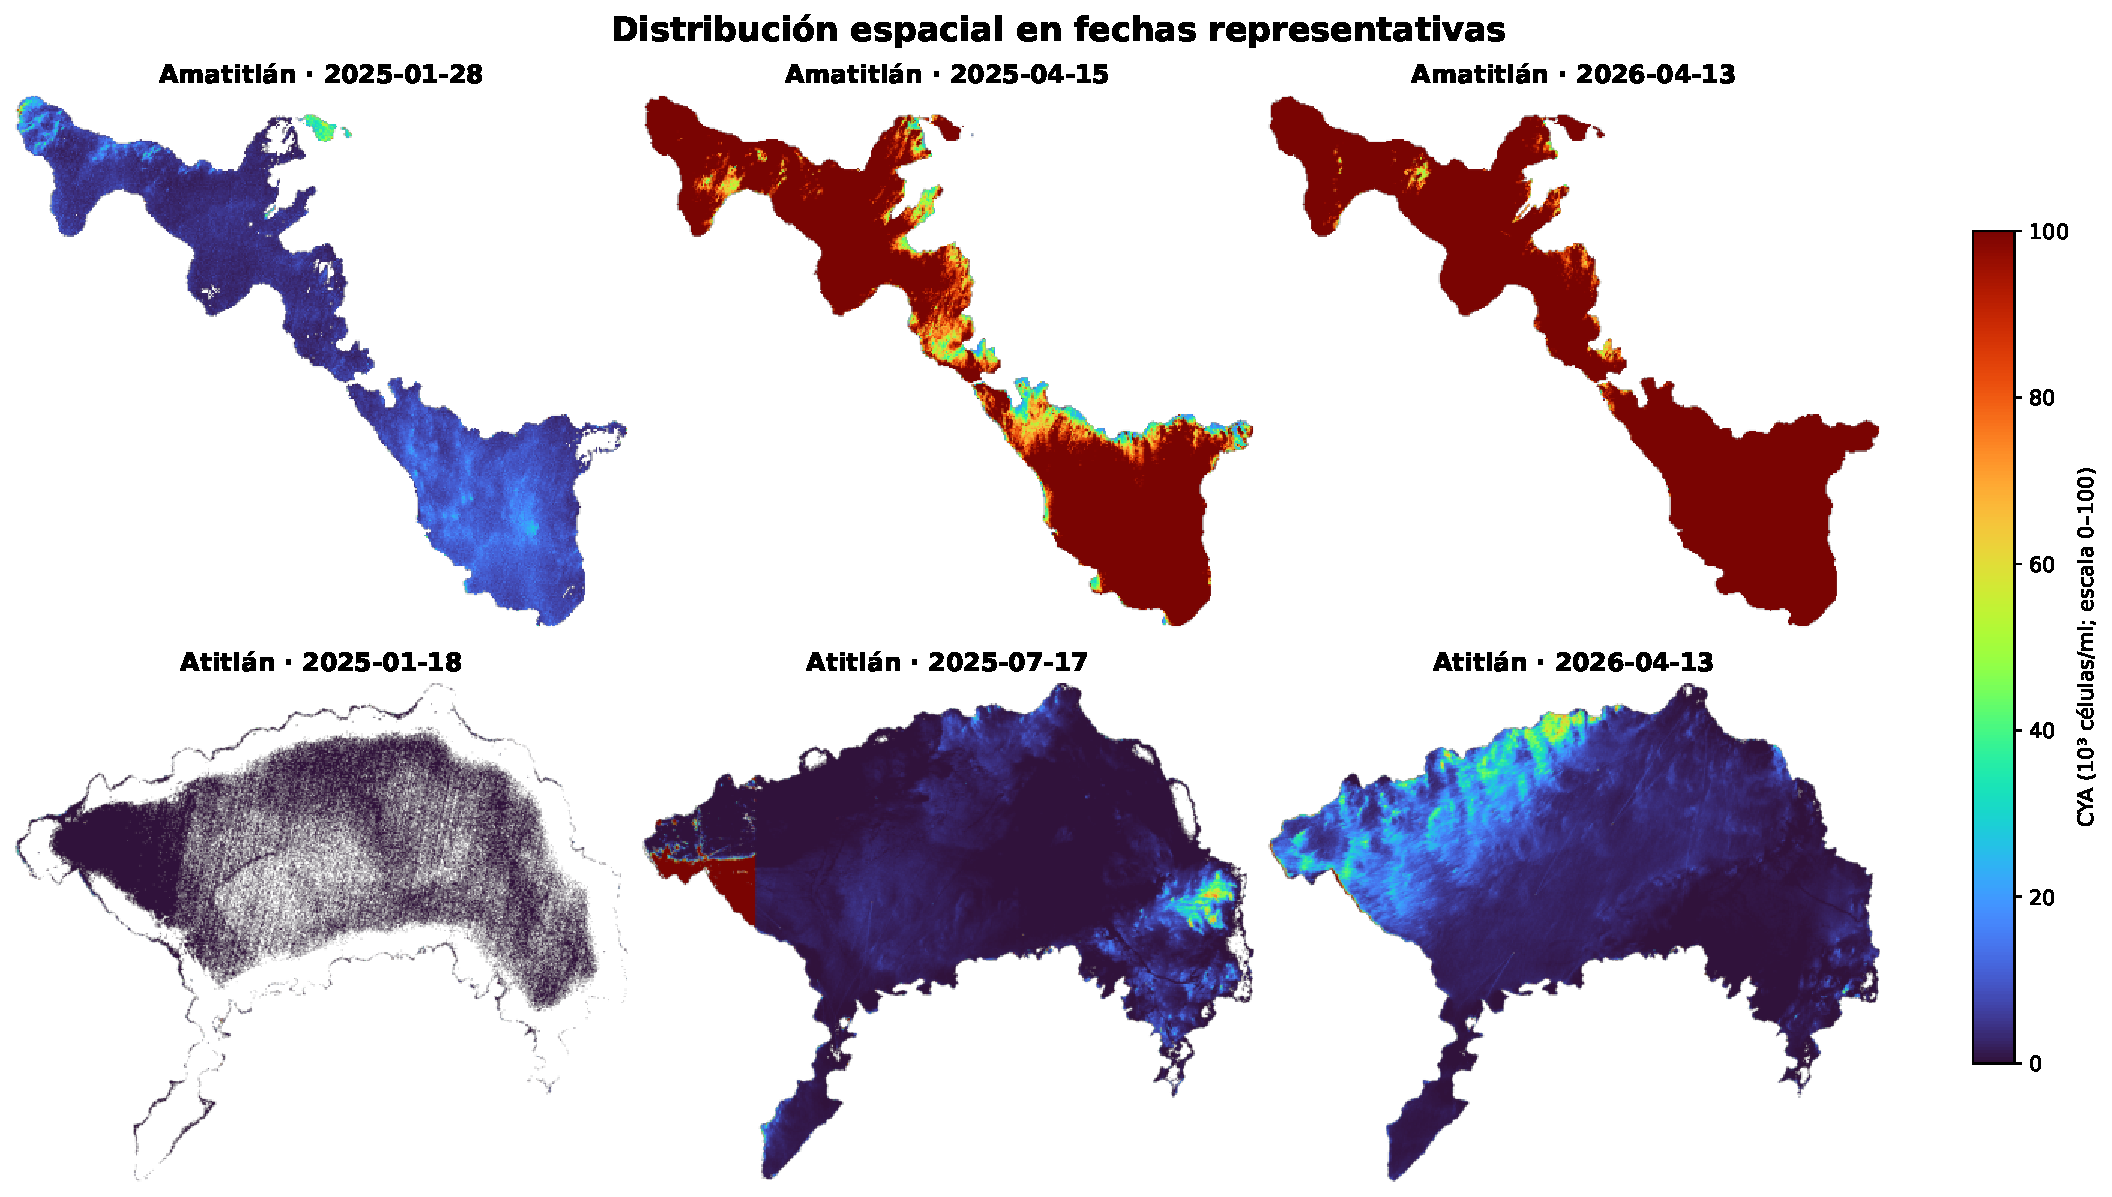
\includegraphics[width=\textwidth]{mapas_cya_seleccion.pdf}
\caption{Distribución espacial en fechas representativas con buena calidad visual. La rampa común 0--100 facilita la comparación; el triángulo superior indica valores que exceden la escala.}
\label{fig:mapas}
\end{figure}

En Amatitlán, las fechas altas no se limitaron a una bahía: ocuparon los dos lóbulos y el canal que los conecta. En el resumen por cuadrantes, el noroeste tuvo la mayor mediana típica (119.37), seguido del sureste (84.08), noreste (77.99) y suroeste (60.03). Las diferencias internas siguen siendo menores que el contraste entre fechas bajas y altas.

Atitlán presentó un fondo generalmente bajo con focos pequeños y cambiantes. La mediana típica por cuadrante varió entre 0.50 y 0.83. Los porcentajes altos fueron mayores en algunos sectores occidentales y surorientales, pero no formaron una cobertura generalizada y parte del máximo occidental de julio de 2025 es un artefacto.

\begin{figure}[H]
\centering
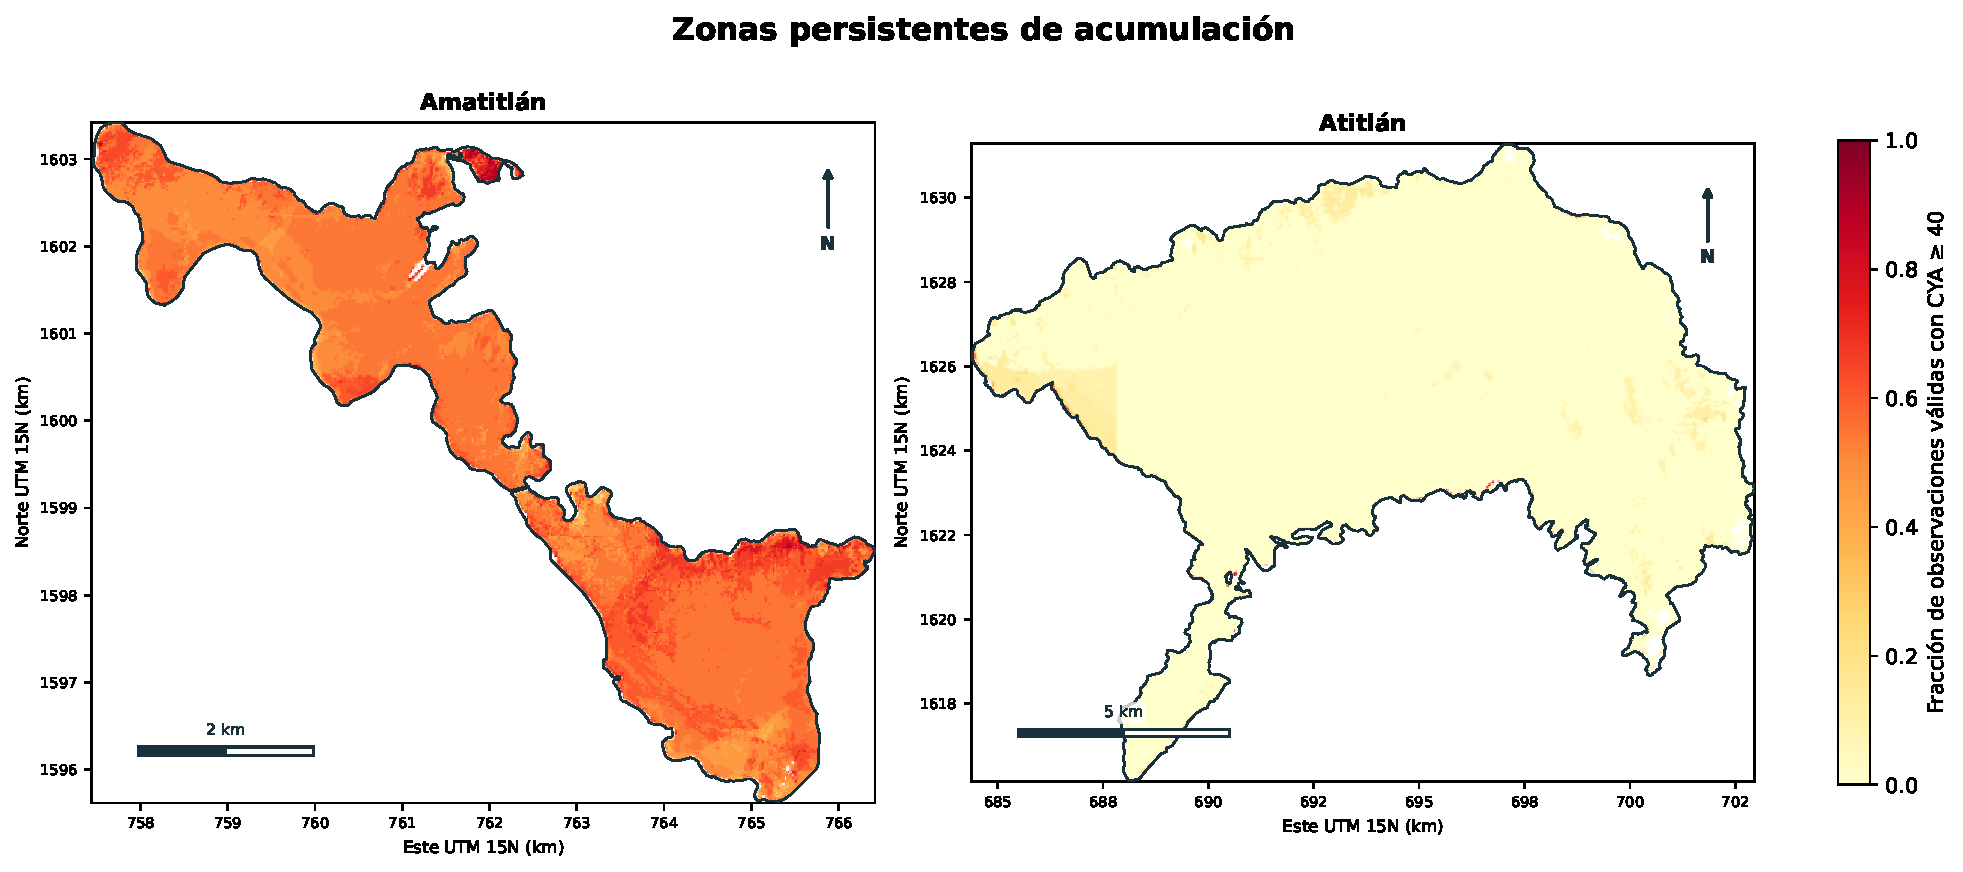
\includegraphics[width=.92\textwidth]{persistencia_cya.pdf}
\caption{Persistencia de \CYA{} $\geq40$. Solo se muestran píxeles con al menos seis observaciones válidas.}
\label{fig:persistencia}
\end{figure}

En Amatitlán, 90.44\% del área superó 40 en al menos la mitad de sus observaciones válidas; 1.38\% lo hizo en al menos tres cuartas partes. En Atitlán estas proporciones fueron 0.20\% y 0.09\%. La persistencia confirma que el contraste no depende de un único día, aunque el denominador variable exige cautela.

\section{Correlación con NDVI y NDWI}

Se calcularon Pearson, Pearson sobre $\log_{10}(\CYA)$ y Spearman por lago y fecha. También se generó una submuestra espacial regular para comprobar la estabilidad del signo sin tratar cada píxel vecino como observación completamente independiente.

\begin{table}[H]
\centering
\caption{Mediana del coeficiente de Spearman entre las once fechas.}
\begin{tabular}{llrr}
\toprule
\textbf{Lago} & \textbf{Relación} & \textbf{Coeficiente mediano} & \textbf{Fechas negativas} \\
\midrule
Amatitlán & CYA--NDVI & 0.324 & 2 de 11 \\
Amatitlán & CYA--NDWI & -0.488 & 9 de 11 \\
Atitlán & CYA--NDVI & 0.078 & 5 de 11 \\
Atitlán & CYA--NDWI & -0.776 & 11 de 11 \\
\bottomrule
\end{tabular}
\end{table}

\begin{figure}[H]
\centering
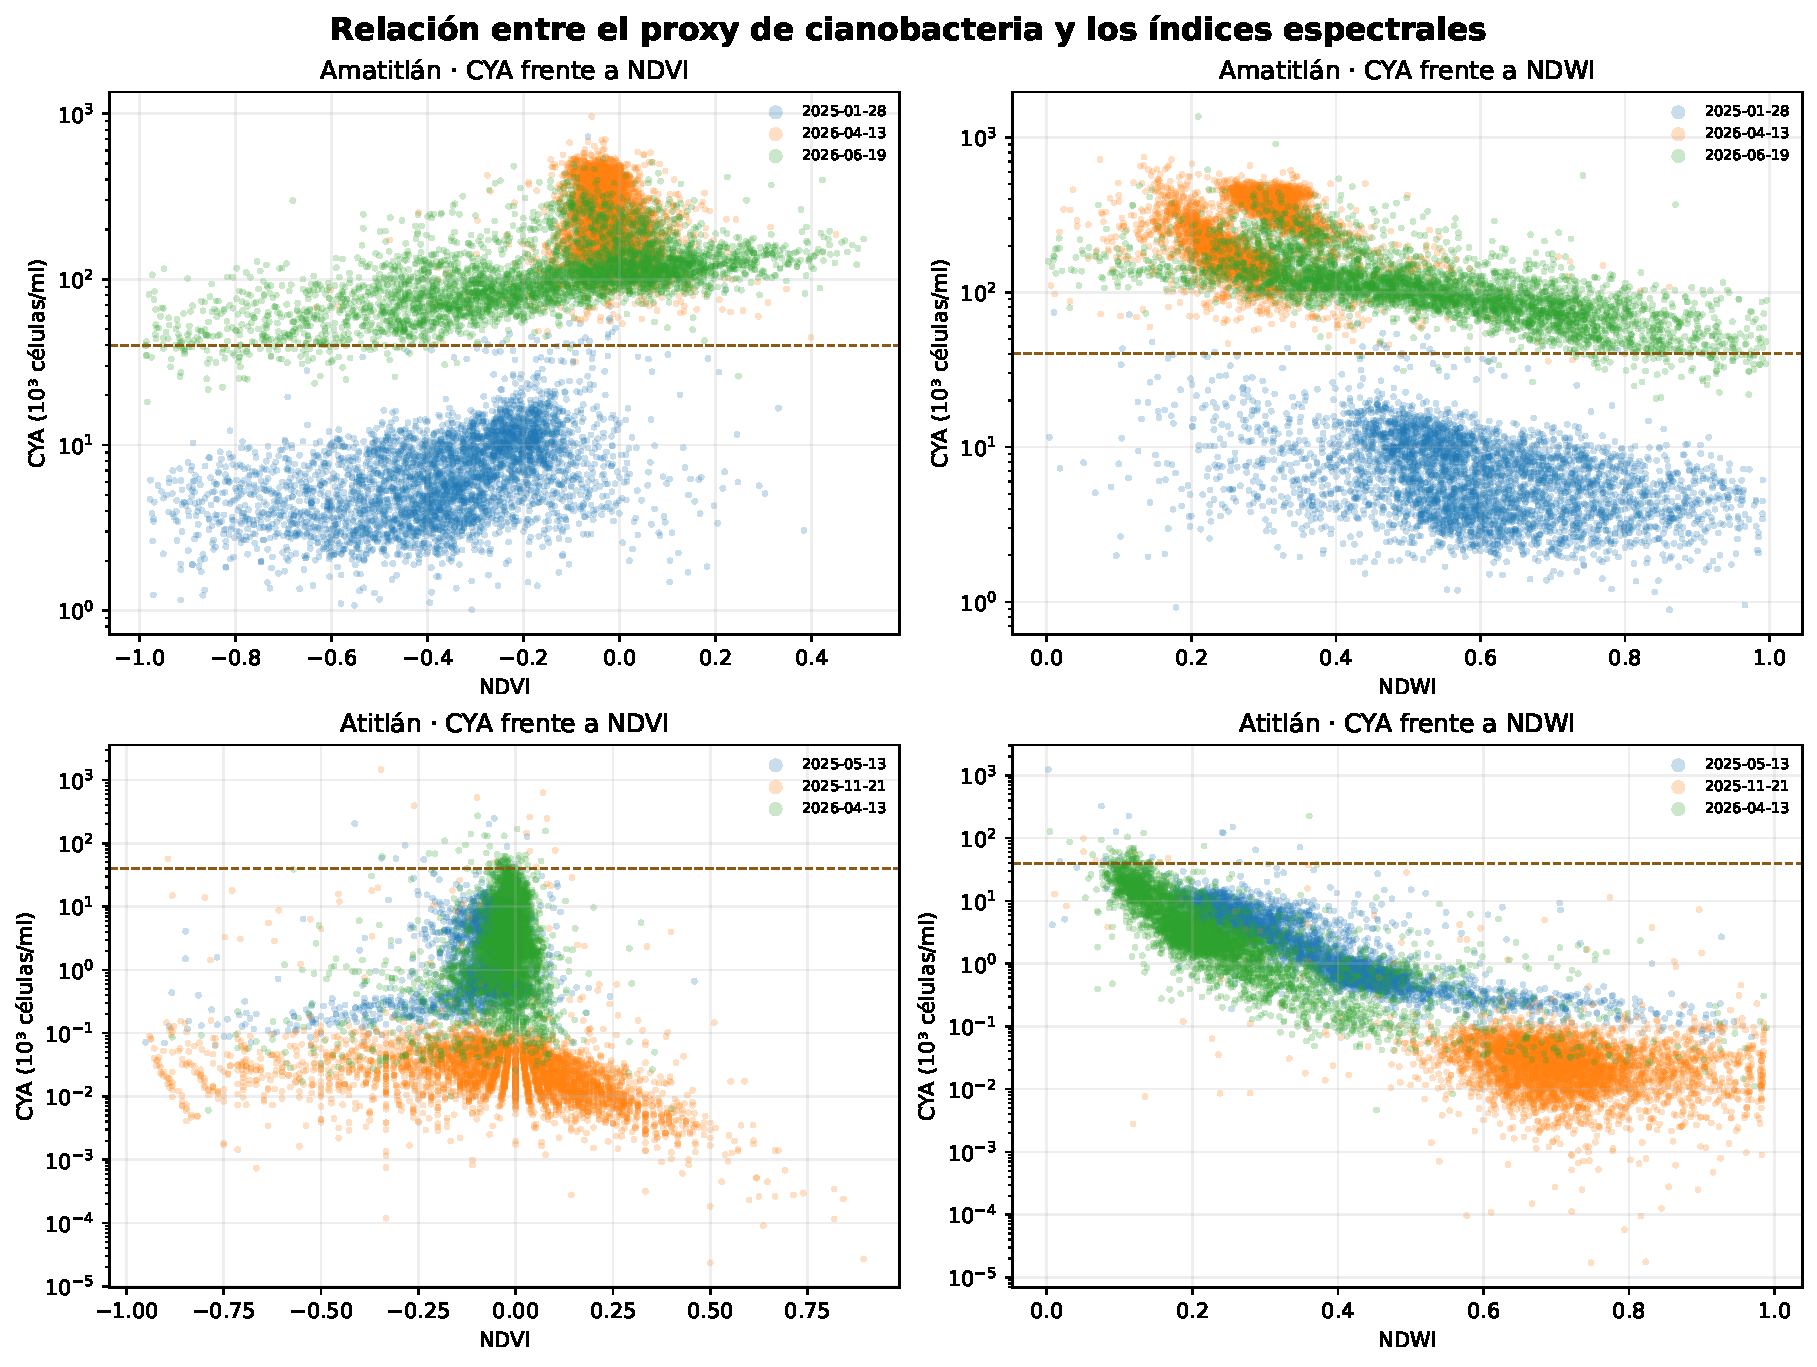
\includegraphics[width=\textwidth]{dispersion_correlaciones.pdf}
\caption{Dispersión entre \CYA{}, NDVI y NDWI en fechas representativas. \CYA{} se muestra en escala logarítmica.}
\end{figure}

La relación con NDVI fue débil en Atitlán y débil a moderada en Amatitlán, además de cambiar de signo en algunas fechas. No existe una correspondencia simple entre vegetación terrestre y el proxy dentro del agua. La relación \CYA{}--NDWI fue predominantemente negativa. Esto no demuestra que más agua reduzca cianobacterias: ambos índices comparten bandas y el propio filtro $\mathrm{NDWI}\geq0$ restringe el dominio. Los valores de significancia estadística son optimistas por autocorrelación espacial y no se usan como prueba causal.

\section{Comparación ambiental de los lagos}

\begin{figure}[H]
\centering
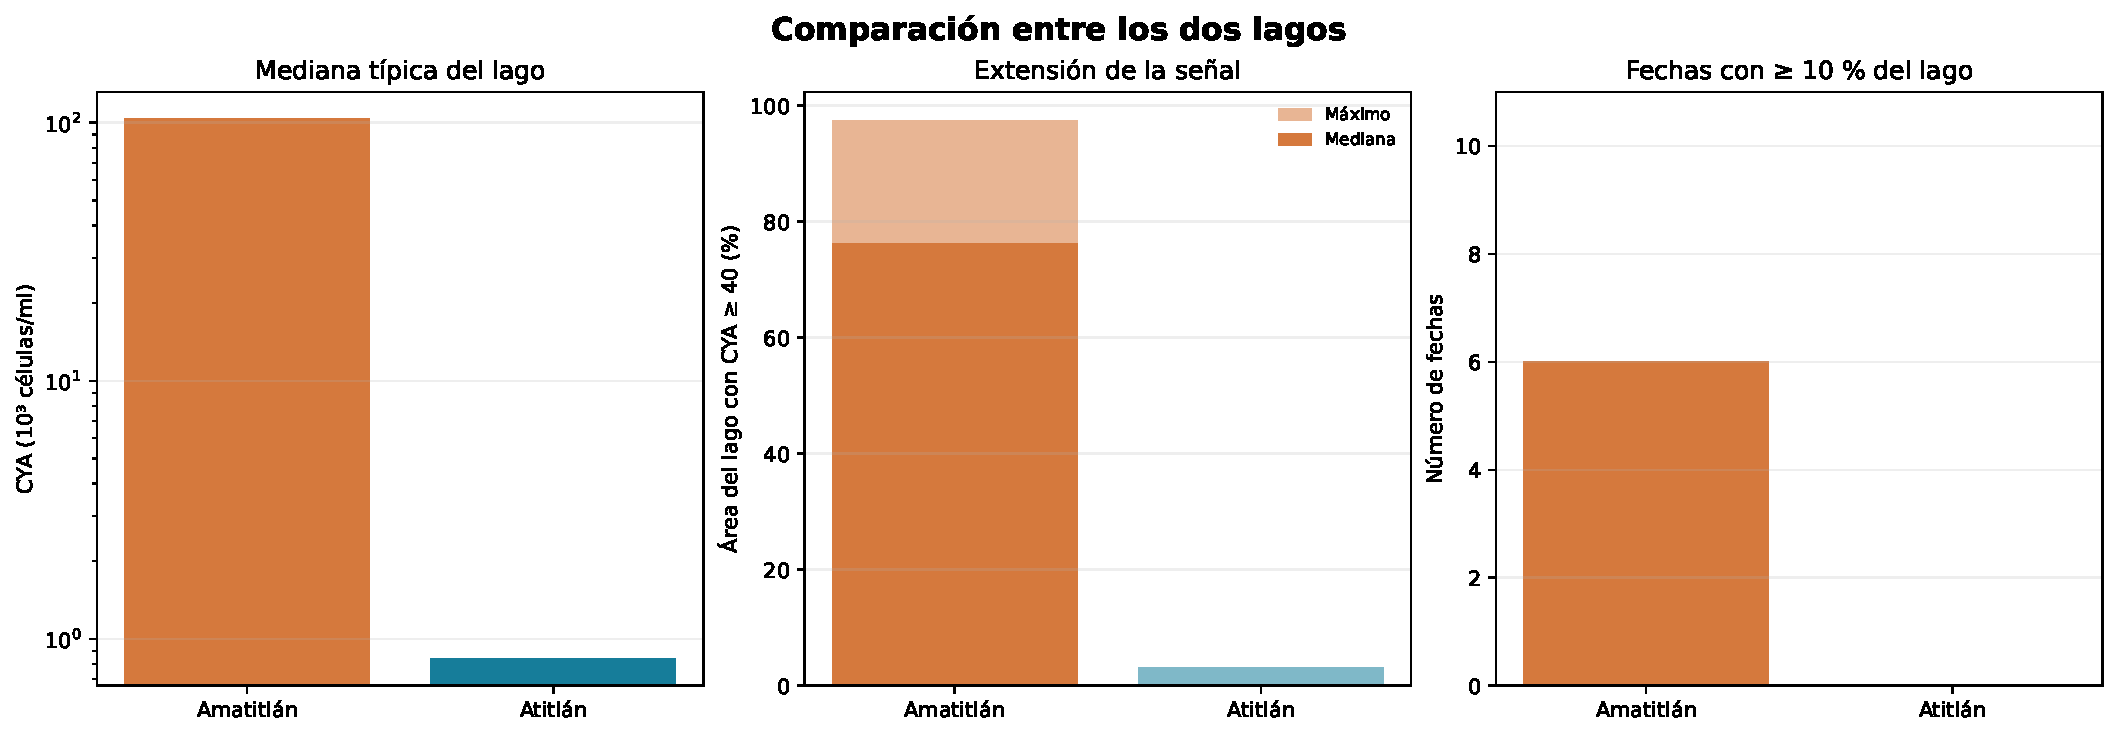
\includegraphics[width=\textwidth]{comparacion_lagos.pdf}
\caption{Comparación de intensidad típica, extensión y frecuencia de fechas críticas.}
\label{fig:comparacion}
\end{figure}

\begin{table}[H]
\centering
\caption{Indicadores principales de comparación.}
\begin{tabular}{lrr}
\toprule
\textbf{Indicador} & \textbf{Amatitlán} & \textbf{Atitlán} \\
\midrule
Mediana típica de CYA & 103.35 & 0.84 \\
Máxima mediana de CYA & 262.24 & 2.57 \\
Mediana del área alta & 76.34\% & 0.21\% \\
Máxima área alta & 97.50\% & 3.14\%$^*$ \\
Fechas críticas & 6 & 0 \\
Área persistente, fracción $\geq0.50$ & 90.44\% & 0.20\% \\
\bottomrule
\end{tabular}

\smallskip
\footnotesize $^*$La imagen asociada contiene una discontinuidad rectangular y no se interpreta como cobertura natural completa.
\end{table}

El contraste de la Figura~\ref{fig:comparacion} es coherente con diferencias en morfología y presión de cuenca. AMSA describe Amatitlán como un lago sometido a contaminación continua, con descargas de municipios de la cuenca y escaso tratamiento \cite{amsa2022}. Estudios sedimentarios relacionan su condición moderna con aportes excesivos de nutrientes transportados por el río Villalobos desde el área metropolitana \cite{waters2021}.

Atitlán es más grande, profundo y endorreico. La literatura documenta aguas residuales sin tratar, erosión y escorrentía agrícola como fuentes de nutrientes \cite{weisman2018,amsclae2024}. También ha tenido floraciones históricas; por ello, la señal menor del período estudiado no implica ausencia de riesgo futuro. Temperatura, mezcla vertical, disponibilidad de nitrógeno y fósforo, viento y precipitación pueden modificar los eventos \cite{amsclae2024}. No se contó con estas variables simultáneas, por lo que son explicaciones plausibles y no causas demostradas por este análisis.

\section{Análisis exploratorio adicional}

\subsection{Sensibilidad del umbral}

El patrón general se mantuvo con umbrales 20, 40 y 60. Por ejemplo, el 13-04-2026 Amatitlán cubrió 97.52\%, 97.50\% y 97.05\%, respectivamente. En Atitlán, esa fecha pasó de 7.76\% con 20 a 1.46\% con 40 y 0.40\% con 60. La magnitud exacta depende del corte, pero la diferencia entre lagos es robusta.

\subsection{Distribuciones y diferencias}

\begin{figure}[H]
\centering
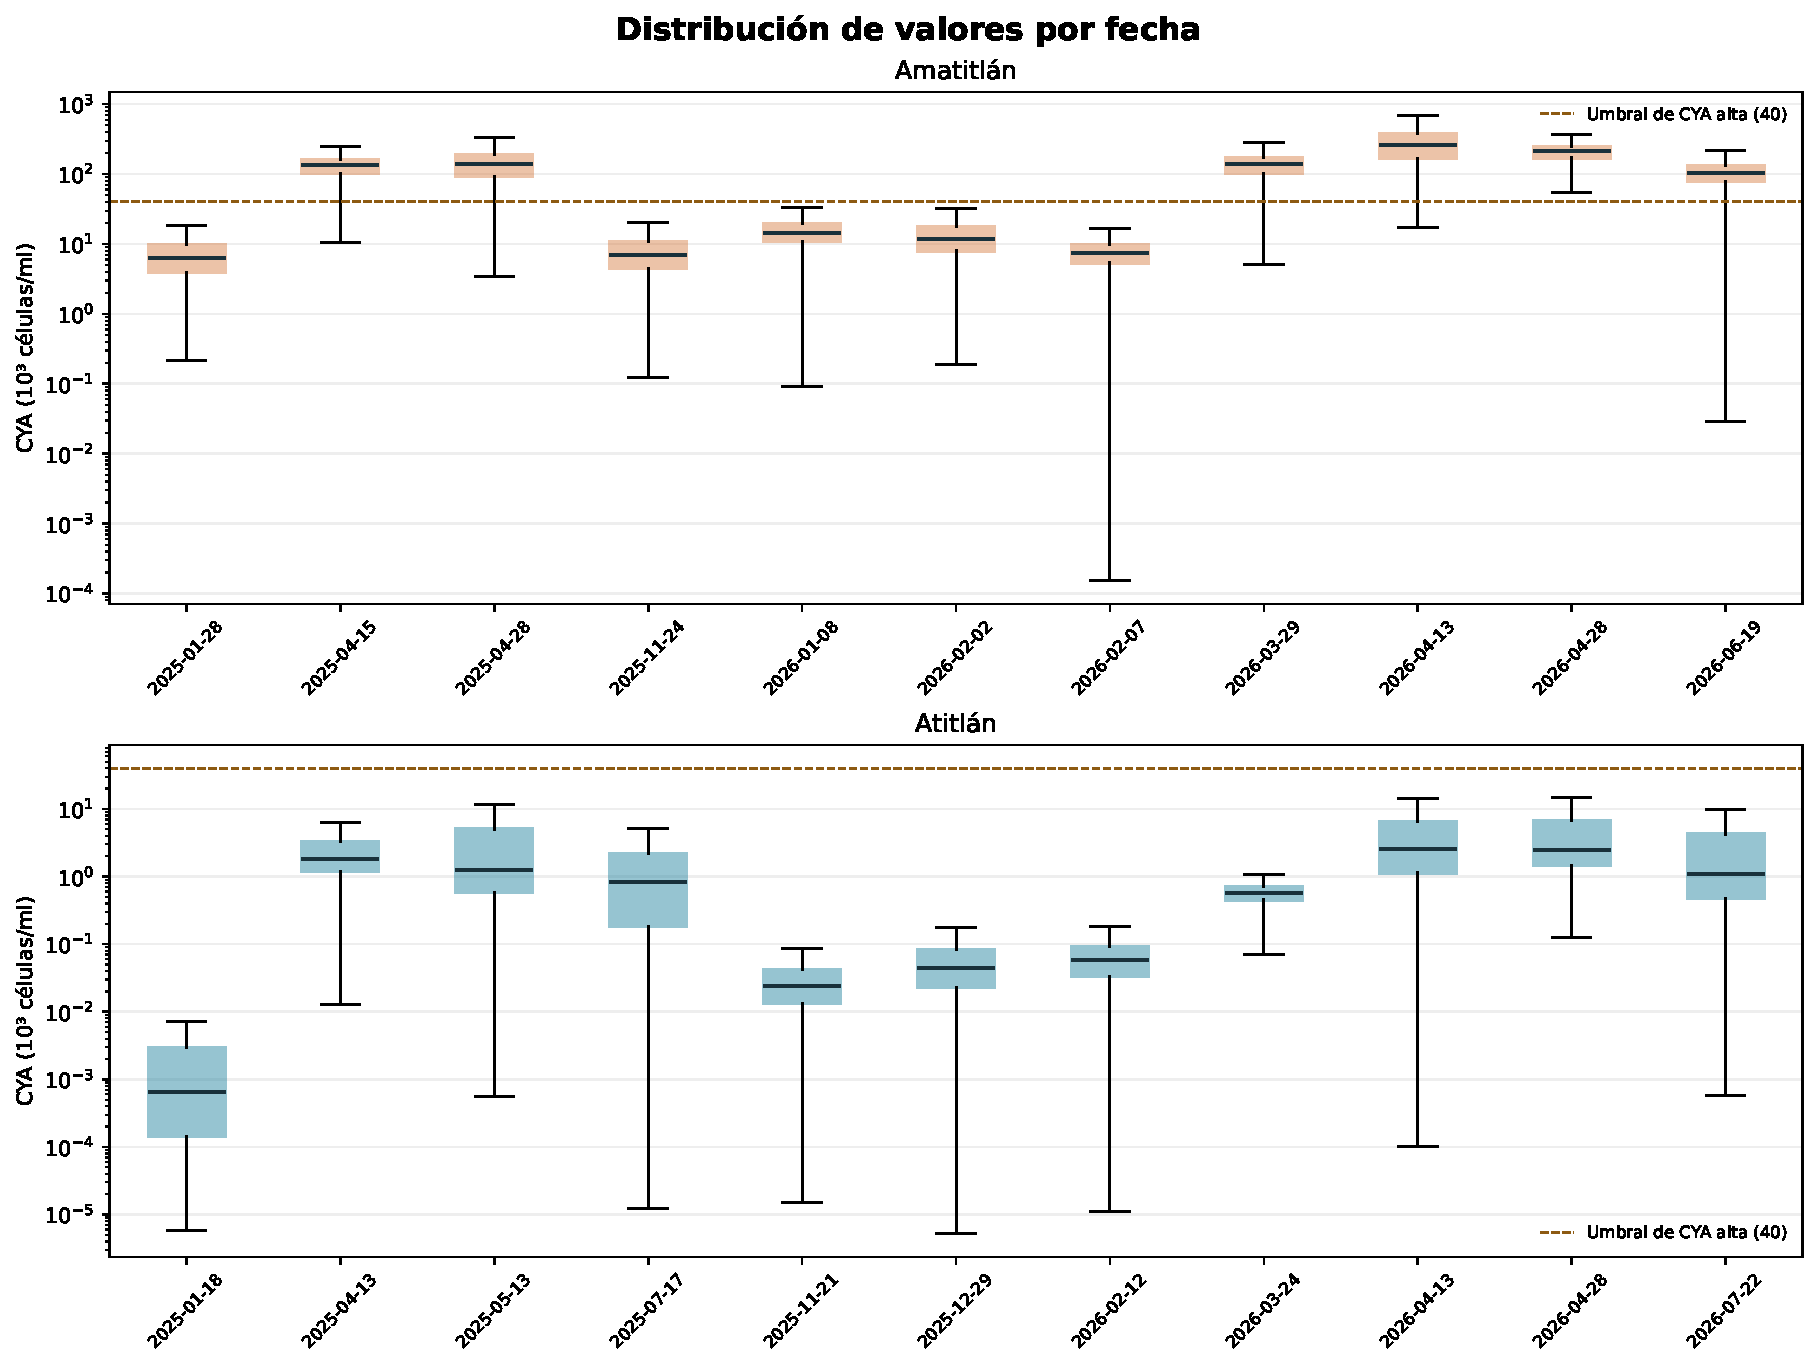
\includegraphics[width=.92\textwidth]{distribuciones_cya.pdf}
\caption{Distribución de \CYA{} por fecha. La escala logarítmica evita que los valores altos oculten la estructura de las fechas bajas.}
\end{figure}

Los boxplots muestran que en Amatitlán no solo aumentaron máximos aislados: durante las fechas críticas se desplazó la distribución completa. En Atitlán, las cajas permanecieron bajas y los valores altos correspondieron principalmente a colas localizadas. Los mapas de diferencia confirman cambios amplios en Amatitlán y cambios puntuales en Atitlán.

\subsection{Exploración estacional}

No puede afirmarse un ciclo estacional. Amatitlán solo tuvo una fecha clasificada como lluviosa, frente a diez secas. Atitlán tuvo tres lluviosas y ocho secas, pero una de las lluviosas contiene el artefacto de julio de 2025. Las medianas exploratorias sugieren señal algo mayor en las fechas lluviosas, pero la muestra es demasiado pequeña e irregular para separar estación, año y eventos individuales.

\section{Limitaciones}

\begin{itemize}
\item Se2WaQ fue calibrado en otro embalse; sus unidades no equivalen a una medición local validada.
\item La regla $\mathrm{NDWI}\geq0$ reproduce el script, pero puede excluir superficies ópticamente semejantes a vegetación, incluidas natas densas.
\item Tres fechas tienen cobertura inferior a 80\% y una presenta una discontinuidad de tesela.
\item No hubo conteos de células, toxinas, nutrientes, temperatura o viento coincidentes con el paso satelital.
\item Los píxeles tienen autocorrelación espacial; un gran número de píxeles no equivale al mismo número de muestras independientes.
\item Las once fechas por lago no forman una serie regular y no permiten atribuir estacionalidad.
\item El umbral de 40 y el criterio de 10\% son reglas exploratorias declaradas, no normas sanitarias.
\end{itemize}

\section{Conclusiones}

\begin{enumerate}
\item Se completó un flujo reproducible que conecta con la API, utiliza los GeoJSON y fechas del curso, solicita bandas mínimas y genera NDVI, NDWI y \CYA{} para las 22 observaciones.
\item Amatitlán mostró señales mucho más intensas, extensas y persistentes. Seis fechas fueron críticas bajo el criterio exploratorio y los máximos se concentraron en abril de 2025 y marzo--junio de 2026.
\item Atitlán presentó valores menores y focos localizados. Ninguna fecha superó 10\% del lago; la mayor mediana ocurrió el 13-04-2026.
\item Las correlaciones no proporcionan un indicador independiente de causalidad. La asociación negativa con NDWI está condicionada por bandas compartidas y la máscara acuática.
\item La diferencia entre lagos es compatible con sus presiones de cuenca y dinámica física, pero solo una campaña de campo simultánea puede confirmar concentración, especie y toxicidad.
\item Los mapas permiten priorizar fechas y zonas para muestreo, especialmente durante aumentos extensos en Amatitlán y focos costeros o localizados en Atitlán.
\end{enumerate}

\section*{Reproducibilidad y materiales}

El análisis completo se regenera con \texttt{python scripts/analyze\_full.py}. El notebook ejecutado es \texttt{notebooks/02\_laboratorio\_completo.ipynb}; las tablas se encuentran en \texttt{outputs/tables} y las figuras, incluidos dos mapas Folium, en \texttt{outputs/figures}. El código versionado está disponible en el \href{https://github.com/DanielBarillasM/Laboratorio-4.-Analisis-Geoespacial-y-sensores-remotos_DS_Grupo-1}{repositorio GitHub del Grupo 1}.

\begin{thebibliography}{9}
\bibitem{se2waq}
Pereira, N. S. A. (2020). \textit{Se2WaQ -- Sentinel--2 Water Quality Script}. Sentinel Hub Custom Scripts. \url{https://custom-scripts.sentinel-hub.com/custom-scripts/sentinel-2/se2waq/}

\bibitem{potes2018}
Potes, M. et al. (2018). \textit{Use of Sentinel 2--MSI for water quality monitoring at Alqueva reservoir, Portugal}. Proceedings of the International Association of Hydrological Sciences, 380, 73--79.

\bibitem{cdse}
Copernicus Data Space Ecosystem. \textit{openEO API documentation}. \url{https://documentation.dataspace.copernicus.eu/APIs/openEO/openEO.html}

\bibitem{amsa2022}
Autoridad para el Manejo Sustentable de la Cuenca y del Lago de Amatitlán. \textit{Plan Estratégico Institucional 2022--2030}. \url{https://pruebas.amsa.gob.gt/wp-content/uploads/2025/04/UTF-84287_16219_1.-Plan-Estrategico-Institucional-2022-2030-31ENE2023.pdf}

\bibitem{waters2021}
Waters, M. N. et al. (2021). \textit{Harmful algal blooms and cyanotoxins in Lake Amatitlán, Guatemala, coincided with ancient Maya occupation in the watershed}. Proceedings of the National Academy of Sciences, 118(48). \url{https://doi.org/10.1073/pnas.2109919118}

\bibitem{amsclae2024}
Autoridad para el Manejo Sustentable de la Cuenca del Lago de Atitlán. (2024). \textit{Informe anual de investigación y calidad ambiental}. \url{https://www.amsclae.gob.gt/wp-content/uploads/2025/02/InformesDICA2024.pdf}

\bibitem{weisman2018}
Weisman, D. et al. (2018). \textit{Effects of nutrient limitations and watershed inputs on community respiration in a deep, tropical lake}. Water Resources Research, 54. \url{https://doi.org/10.1029/2017WR021981}

\bibitem{osm}
OpenStreetMap contributors. Relaciones 5781818 y 11018382. Datos bajo licencia ODbL 1.0. \url{https://www.openstreetmap.org/copyright}
\end{thebibliography}

\end{document}
